\chapter{Data and Simulated Samples}\label{sec:data}

The data sample used for the CMS Run 2 \hzg{} search corresponds to a total integrated luminosity of \LumiT\fbinv and was collected over a data-taking period spanning three years: \Lumia\fbinv in 2016, \Lumib\fbinv in 2017, and \Lumic\fbinv in 2018~\cite{CMS-LUM-17-003,LUM-17-004,LUM-18-002}. 
To be considered in the analysis, events must satisfy the HLT requirements for at least one of the dielectron or dimuon triggers.
The dielectron trigger requires a leading (subleading) electron with
$\pt > 23\,(12)\GeV$, while the dimuon trigger requires a leading (subleading) muon with $\pt > 17\,(8)\GeV$.
The corresponding CMS data streams are listed in Table~\ref{tab:data_samples}. All data samples use the CMS MINIAOD data format.
To ensure data quality, luminosity masks are applied based on recommendations from the Physics Performance and Dataset group.

\begin{table}[tb]
  \begin{center}
	  \caption{Summary of MINIAOD data samples used.}
    \begin{tabular}{|l|l|}
      \hline
	    \textbf{$\Pe^+\Pe^-\PGg$ final state} & \textbf{$\PGm^+\PGm^+\PGg$ final state}	                     \\\hline 
      /DoubleEG/Run2016B-17Jul2018\_ver2-v1 	&  /DoubleMuon/Run2016B-17Jul2018\_ver2-v1   \\
      /DoubleEG/Run2016C-17Jul2018-v1 		&  /DoubleMuon/Run2016C-17Jul2018-v1         \\
      /DoubleEG/Run2016D-17Jul2018-v1 		&  /DoubleMuon/Run2016D-17Jul2018-v1         \\
      /DoubleEG/Run2016E-17Jul2018-v1	        &  /DoubleMuon/Run2016E-17Jul2018-v1         \\       
      /DoubleEG/Run2016F-17Jul2018-v1	        &  /DoubleMuon/Run2016F-17Jul2018-v1         \\       
      /DoubleEG/Run2016G-17Jul2018-v1	        &  /DoubleMuon/Run2016G-17Jul2018-v1         \\
      /DoubleEG/Run2016H-17Jul2018-v1	        &  /DoubleMuon/Run2016H-17Jul2018-v1         \\
      /DoubleEG/Run2016H-17Jul2018-v1	        &  /DoubleMuon/Run2016H-17Jul2018-v1         \\
      /DoubleEG/Run2017B-31Mar2018-v1	        &  /DoubleMuon/Run2017B-31Mar2018-v1         \\
      /DoubleEG/Run2017C-31Mar2018-v1	        &  /DoubleMuon/Run2017C-31Mar2018-v1         \\
      /DoubleEG/Run2017D-31Mar2018-v1	        &  /DoubleMuon/Run2017D-31Mar2018-v1         \\
      /DoubleEG/Run2017E-31Mar2018-v1	        &  /DoubleMuon/Run2017E-31Mar2018-v1         \\       
      /DoubleEG/Run2017F-31Mar2018-v1	        &  /DoubleMuon/Run2017F-31Mar2018-v1         \\           
      /EGamma/Run2018A-17Sep2018-v2		&  /DoubleMuon/Run2018A-17Sep2018-v2         \\  
      /EGamma/Run2018B-17Sep2018-v1		&  /DoubleMuon/Run2018B-17Sep2018-v1         \\
      /EGamma/Run2018C-17Sep2018-v1		&  /DoubleMuon/Run2018C-17Sep2018-v1         \\
      /EGamma/Run2018D-22Jan2019-v2		&  /DoubleMuon/Run2018D-PromptReco-v2        \\\hline       
    \end{tabular}
    \label{tab:data_samples}
  \end{center}
\end{table}

Signal samples for $\Pg\Pg\PH$, VBF, $\mathrm{V}\PH$, and $\ttbar\PH$ production, with 
$\PH\to\PZ\gamma$ and $\PZ\to\ell^+\ell^-$ ($\ell = \Pe$, $\mu$, or $\tau$),
are generated at next-to-leading order (NLO) using \POWHEG v2.0~\cite{cite:powheg1,cite:powheg2}.
These samples are produced for $m_\PH$ of $120$, $125$, and $130$\GeV. 
The dominant backgrounds, $\PZ/\gamma^{*}(\rightarrow \ell^+\ell^-)$+$\gamma$ and $\PZ/\gamma^{*}(\rightarrow \ell^+\ell^-)$+jets,
are generated at NLO using the \MGvATNLO v2.6.0 (v2.6.1) 
generator~\cite{Alwall:2014hca} for 2016 (2017 and 2018) samples. 
 Events arising from $\ttbar$ production~\cite{Frixione:2007nw} are a relatively minor background and are generated at NLO with \POWHEG v2.0~\cite{cite:powheg1,cite:powheg2}.
 The background from vector boson scattering (VBS) production of $\PZ/\gamma^{*}$+$\gamma$ pairs, with the $\PZ$ boson decaying to a pair of leptons, is simulated at leading order using the \MGvATNLO generator. The decay $\PH\to\mpmm$ is considered as a resonant background and is generated for the $\Pg\Pg\PH$, VBF,  $\mathrm{V}\PH$, and $\ttbar\PH$ production mechanisms. The $\Pg\Pg\PH$ production cross section is
computed at next-to-next-to-NLO precision in QCD and at NLO in electroweak (EWK)
theory~\cite{Anastasiou:2016cez}. 
The cross sections for Higgs boson production in the VBF~\cite{PhysRevLett.115.082002} and VH~\cite{BREIN2004149} mechanisms are calculated at next-to-NLO in QCD, including NLO EWK corrections, while the $\ttbar\PH$ cross section is computed at NLO in QCD and EWK theory~\cite{PhysRevD.68.034022}. 

A full list of simulated physics processes used in the analysis is provided in Table~\ref{tab:sim_samples}, along with cross section and branching fraction information. 
For the \hzg{} and $\PH\to\mpmm$ samples, the SM Higgs boson production cross sections and branching fractions
recommended by the LHC Higgs Working
Group~\cite{LHC-YR4} are used for each mass point.
The values for the Higgs boson processes listed in Table~\ref{tab:sim_samples} correspond to $m_{\PH}=125\GeV$.

\begin{table}[tb]
	\begin{center}
		\caption{Simulated event samples used in the analysis. For Higgs samples, the listed cross sections and branching fractions correspond to the values for $m_{\PH}=125\GeV$. In this table, $\ell$ denotes $\Pe$, $\mu$, or $\tau$.}
		\begin{tabular}{|l|c|c|}
			\hline
			\textbf{process} & \textbf{cross section (pb)} & \textbf{branching fraction}\\\hline 
			$\mathrm{gg}\PH\to\PZ\gamma\to\lplm\gamma$ & 48.58 & $1.548\times 10^{-3}$ \\ 
			$\mathrm{q\bar{q}}\PH\to\PZ\gamma\to\lplm\gamma$ & 3.782 & $1.548\times 10^{-3}$\\
			$\PZ\PH\to\PZ\gamma\to\lplm\gamma$ & 0.8839 & $1.548\times 10^{-3}$\\ 
			$\PW^+\PH\to\PZ\gamma\to\lplm\gamma$ & 0.84 & $1.548\times 10^{-3}$\\
			$\PW^-\PH\to\PZ\gamma\to\lplm\gamma$ & 0.532 & $1.548\times 10^{-3}$\\ 
			$\ttbar\PH\to\PZ\gamma\to\lplm\gamma$ & 0.5071 & $1.548\times 10^{-3}$\\ 
			$\mathrm{gg}\PH\to\mpmm$ & 48.58 & $2.176\times 10^{-4}$\\ 
			$\mathrm{q\bar{q}}\PH\to\mpmm$ & 3.782 & $2.176\times 10^{-4}$\\
			$\PZ\PH\to\mpmm$ & 0.8839 & $2.176\times 10^{-4}$\\ 
			$\PW^+\PH\to\mpmm$ & 0.84 & $2.176\times 10^{-4}$\\
			$\PW^-\PH\to\mpmm$ & 0.532 & $2.176\times 10^{-4}$\\ 
			$\ttbar\PH\to\mpmm$ & 0.5071 & $2.176\times 10^{-4}$\\ 
			$\PZ/\gamma^*\to\lplm\gamma$ & 117.864 & --\\
			$\PZ/\gamma^*\to\lplm$+jets & 6225.42 & --\\
			$\ttbar$ (inclusive) & 831.76 & --\\
			VBF $\PZ/\gamma^*+\gamma$ & 0.1097 & --\\

			\hline
		\end{tabular}
		\label{tab:sim_samples}
	\end{center}
\end{table}

All simulated events are interfaced
with \PYTHIA v8.226~(v8.230)~\cite{Sjostrand:2014zea} with the
CUETP8M1~\cite{Khachatryan:2015pea} (CP5~\cite{Sirunyan:2019dfx}) underlying event tune for 2016 (2017--2018) for the
fragmentation and hadronization of partons and the internal bremsstrahlung of the leptons. The NLO parton distribution function (PDF) set, NNPDF v3.0~\cite{nnpdf30}~(NNPDF v3.1)~\cite{nnpdf_new}, is used to produce these samples in 2016 (2017--2018). The response of the CMS detector is modeled using the
\GEANTfour  program~\cite{AGOSTINELLI2003250}. 
The simulated events are reweighted to correct for differences between data and simulation in the number of additional $\Pp\Pp$ interactions, trigger efficiencies, selection efficiencies, and efficiencies of isolation requirements for photons, electrons, and muons. These corrections and their associated uncertainties will be described in more detail throughout the remainder of this thesis. The rest of this chapter will discuss general procedures and corrections related to the data and simulated samples.

\section{Z+jets Overlap Removal}
The two dominant backgrounds in this analysis are $\PZ/\gamma^{*}(\rightarrow \ell^+\ell^-)$+$\gamma$, or $\PZ\gamma$ for short, and $\PZ/\gamma^{*}(\rightarrow \ell^+\ell^-)$+jets, or $\PZ$+jets for short. Both processes 
are simulated independently in order to obtain the best model of the kinematics of the $\lplm\gamma$ system. 
The $\PZ\gamma$ sample simulates photons from initial-state and final-state radiation at the matrix element level and includes a better 
computation of the interference between the corresponding Feynman diagrams than the $\PZ$+jets sample.
However, the $\PZ$+jets
simulated sample also includes the contribution from $\PZ\gamma$. Therefore, this contribution must be removed from the 
$\PZ$+jets sample in order to avoid double counting events and to utilize the better kinematic modeling of the $\PZ\gamma$
sample. To handle this, $\PZ$+jets events are removed from the analysis if they contain prompt, final state photons within 
$\DR = \sqrt{\smash[b]{(\Delta\phi)^2 + (\Delta\eta)^2}} = 0.1$ of the photon selected to reconstruct the $\lplm\gamma$ system.
The events with prompt, final state photons are tagged using generator-level truth information.

\section{Photon Internal Conversion}
\label{sec:gconversion}
The \PYTHIA 8 showering algorithm automatically 
includes a component in which photons from \hgg{} are
internally converted via the process $\PH\to\gamma\gamma^*\to \mathrm{f\bar{f}}\gamma\gamma$, with $\mathrm{f\bar{f}}$ mostly $\epem$. 
This also affects the \hzg{} signal and $\PZ\gamma$ background samples. 
Since the normalization of these samples does not include the internal conversion component, the cross section must be adjusted accordingly.
To determine the amount by which the cross section is adjusted, we calculate the internal conversion
rate in simulation. 
We define a ratio where the numerator is the number of events with hard process final state photons
and the denominator is total number of events in the simulation. Subtracting this ratio from unity gives the internal conversion rate.
The hard process final state photon flagging is done using generator-level truth information.
In our analysis, the internal conversion rate is about 3.1\% (2016) and 3.0\% (2017 and 2018).  
We, consequently, divide the affected sample cross sections by 0.969 (0.97) for 2016 (2017 and 2018).

\section{Transverse Momentum Reweighting}\label{sec:Zpt}
The underlying event tuning was updated from CUETP8M1 (2016) to CP5 (2017--2018). Unfortunately, 
it was discovered that this update caused significant mismodeling of the $\lplm\gamma$ \pt spectrum in the 
$\PZ\gamma$ and $\PZ$+jets background samples in 2017 and 2018. Figure~\ref{fig:pt_reweight} (left) shows the clear difference between 
simulated $\pt^{\lplm\gamma}$ in 2016 and 2017--2018. As will be described later in this thesis, 
the variable $\pt^{\lplm\gamma}/m_{\lplm\gamma}$ has good discriminating power between signal and background and is a useful feature for MVA training.
Therefore, it is important to correct this discrepancy. To do this, a simple reweighting of the distribution is performed using two 
sideband regions in $m_{\lplm\gamma}$. The sidebands are defined as 115--120 and 130--135\GeV. The resulting weights are then applied to 
the $\PZ\gamma$ and $\PZ$+jets simulated events in 2017 and 2018. Figure~\ref{fig:pt_reweight} (right) shows the final distribution of 
$\pt^{\lplm\gamma}/m_{\lplm\gamma}$ for all data-taking years combined after the $\pt^{\lplm\gamma}$ reweighting is applied. The overall agreement 
between data and simulation is good over the full $\pt$ spectrum.

\begin{figure}[tb]
	\begin{center}
		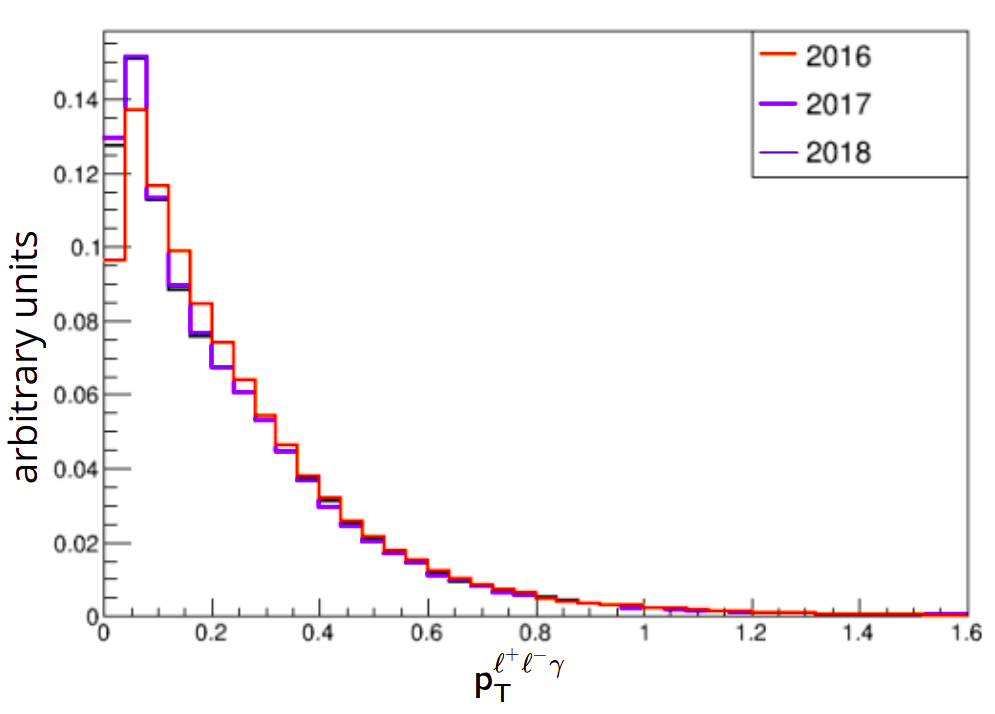
\includegraphics[width=0.45\textwidth, height=0.35\textwidth]{fig/zpt_reweight/ptm_year_comp.png}
		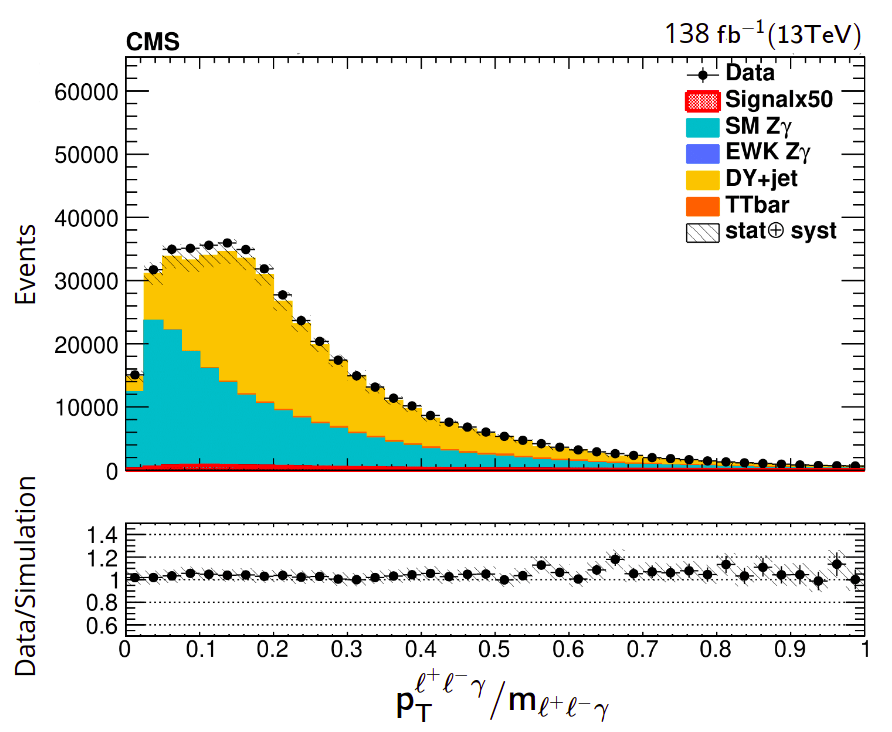
\includegraphics[width=0.45\textwidth, height=0.35\textwidth]{fig/zpt_reweight/pt_over_m_data_mc.png}
	\end{center}
	\caption{Left: Background simulation modeling of $\pt^{\lplm\gamma}$ in each data-taking year. There is a shape discrepancy between 2016 and 2017--2018 due to the 
	updated underlying event tuning. Right: Final comparison between data and simulation after the $\pt^{\lplm\gamma}$ reweighting is performed on 2017 and 2018 background simulation.}
	\label{fig:pt_reweight}
\end{figure}

\section{Pileup Reweighting}\label{sec:pileup}
In order to correctly model the pileup distribution in data, a pileup reweighting procedure must be applied to the simulation.
Although the Deterministic Annealing primary vertex (PV) reconstruction~\cite{detanneal} has been shown to
be efficient and well-behaved up to the observed levels of pileup, the final distribution
for the number of reconstructed PVs is still sensitive to differences between data and 
simulation in the PV reconstruction and underlying event.
Additionally, the offline event selection criteria and trigger can potentially impact the distribution for the number of
reconstructed vertices. 
To handle this, the pileup distribution for data is first derived by using the per-bunch-crossing, per-luminosity-section instantaneous luminosity, 
together with the total pp inelastic cross section. The total pp inelastic cross 
section is taken to be 66 mb, 72.4 mb, and 80 mb for 2016, 2017, and 2018 respectively.
This yields an expected pileup distribution, correctly weighted over the entire data-taking period. The simulation is then reweighted to 
match this expected pileup distribution. 
Figure~\ref{fig:puwei} shows the number of PV after pileup reweighting for each data-taking year. The uncertainties associated with pileup reweighting are 
accounted for in the analysis and are discussed further in Chapter~\ref{sec:uncertainties}.
\begin{figure}[tb]
  \begin{center}
     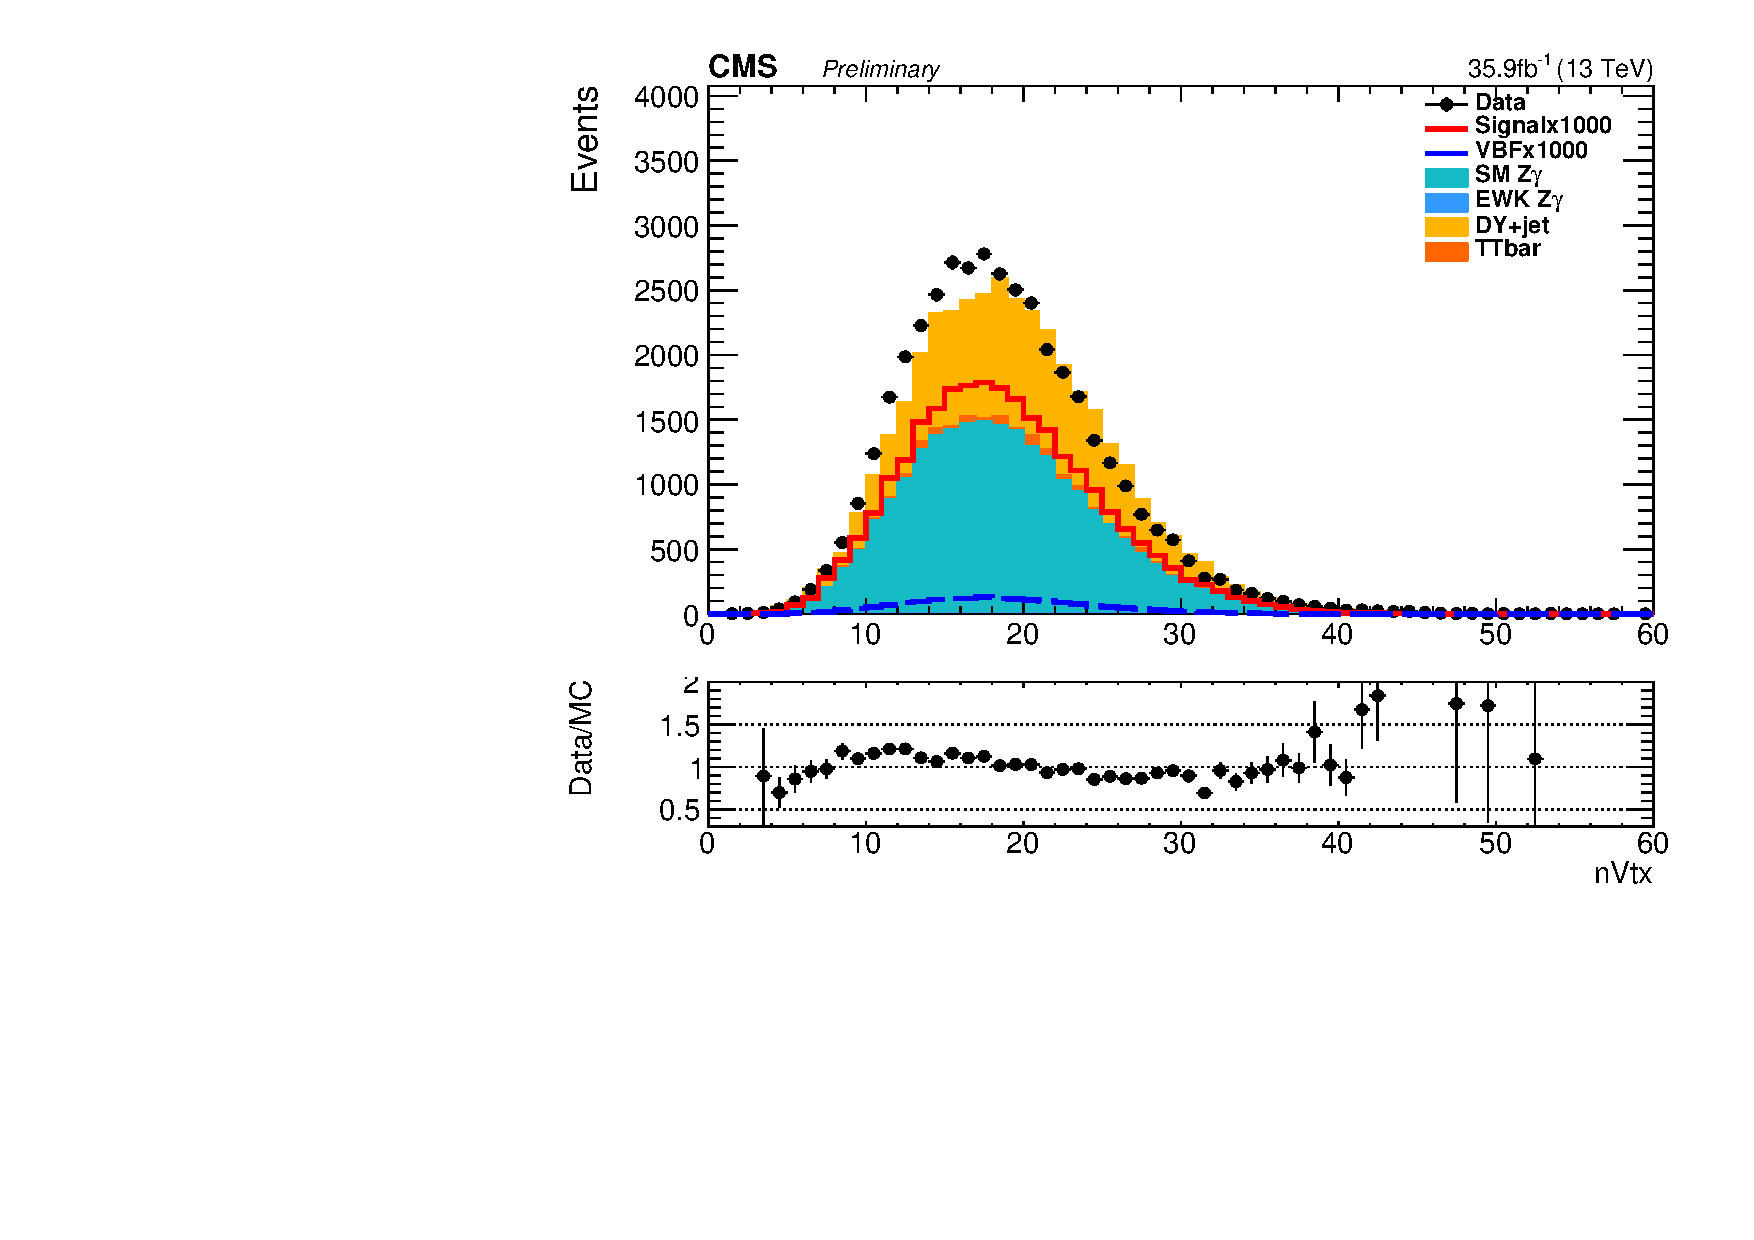
\includegraphics[width=0.3\textwidth]{fig/pileup/ele_kin_nVtx_valid_Legacy16_HLT.pdf}
     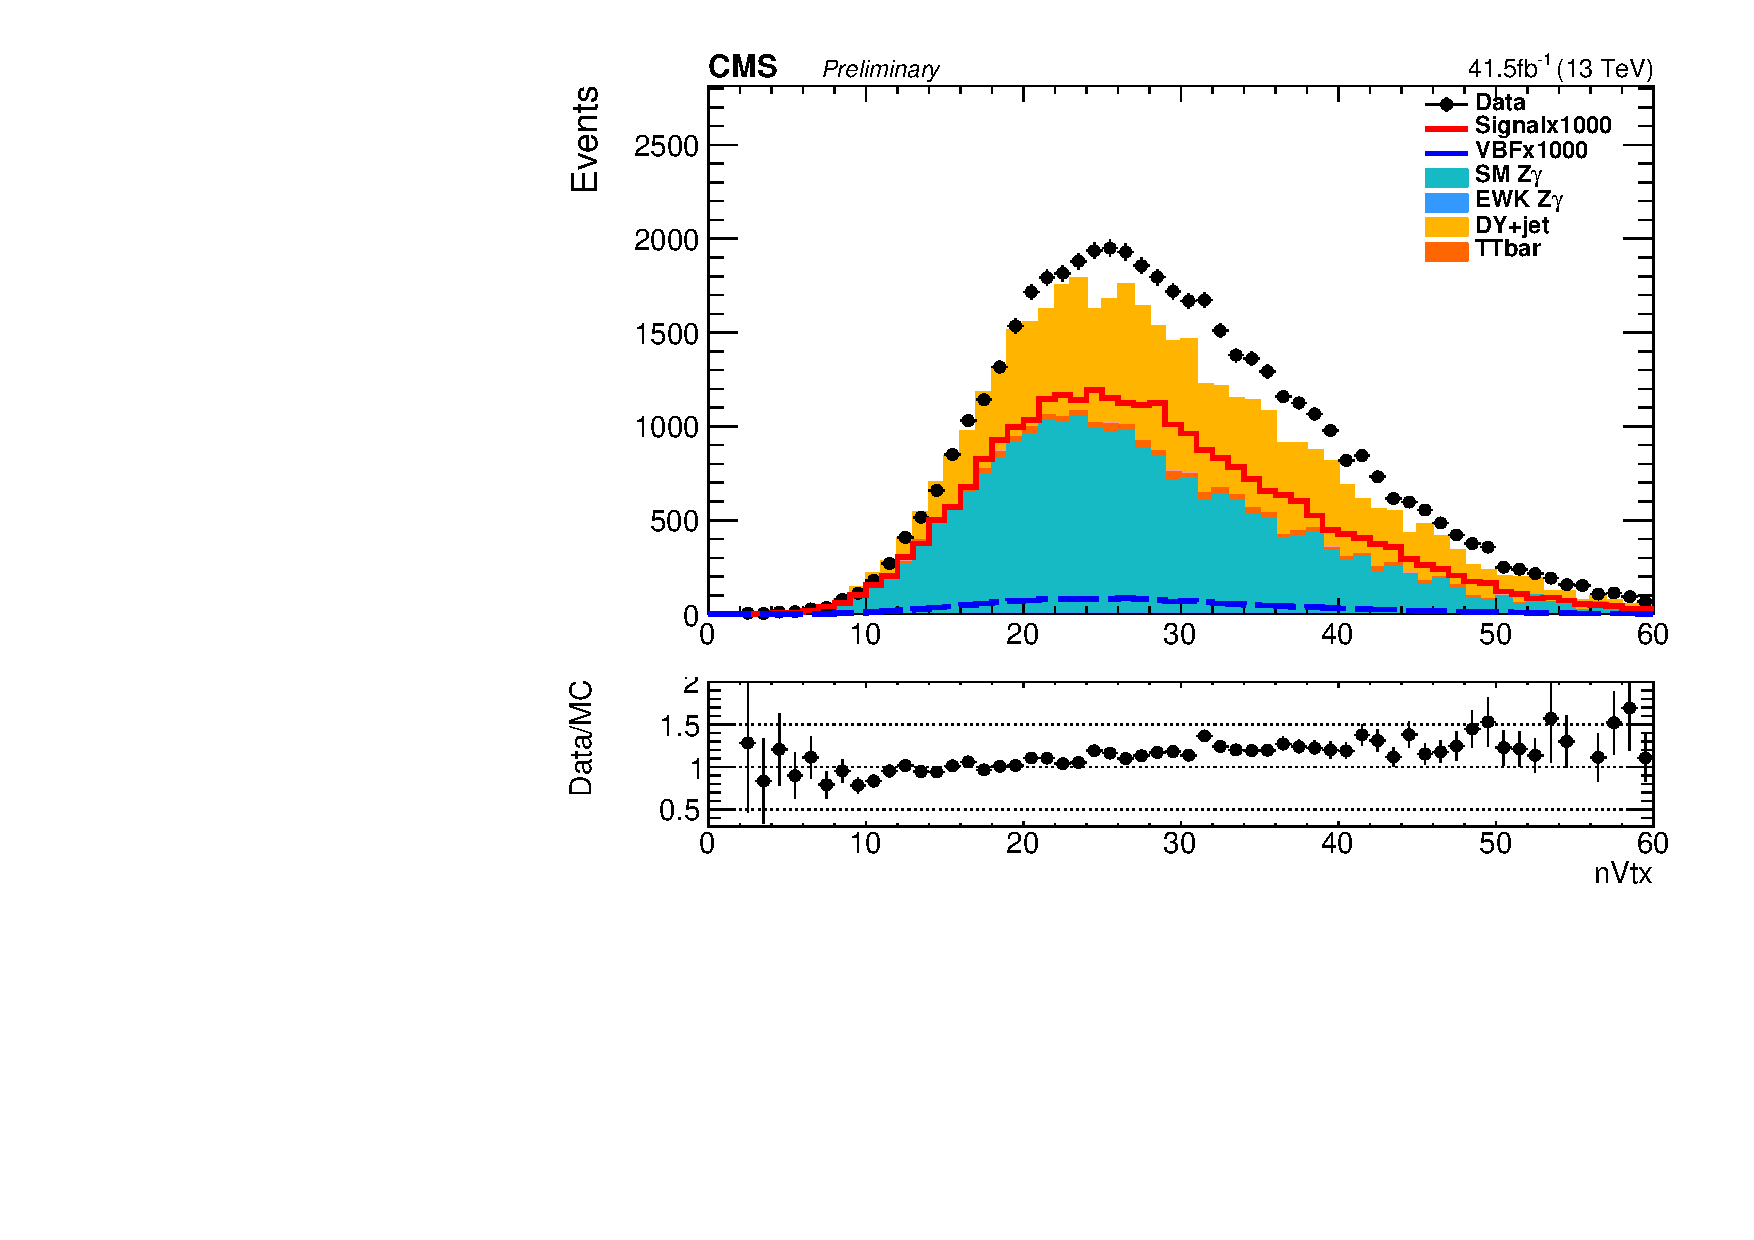
\includegraphics[width=0.3\textwidth]{fig/pileup/ele_kin_nVtx_valid_Rereco17_HLT.pdf}
     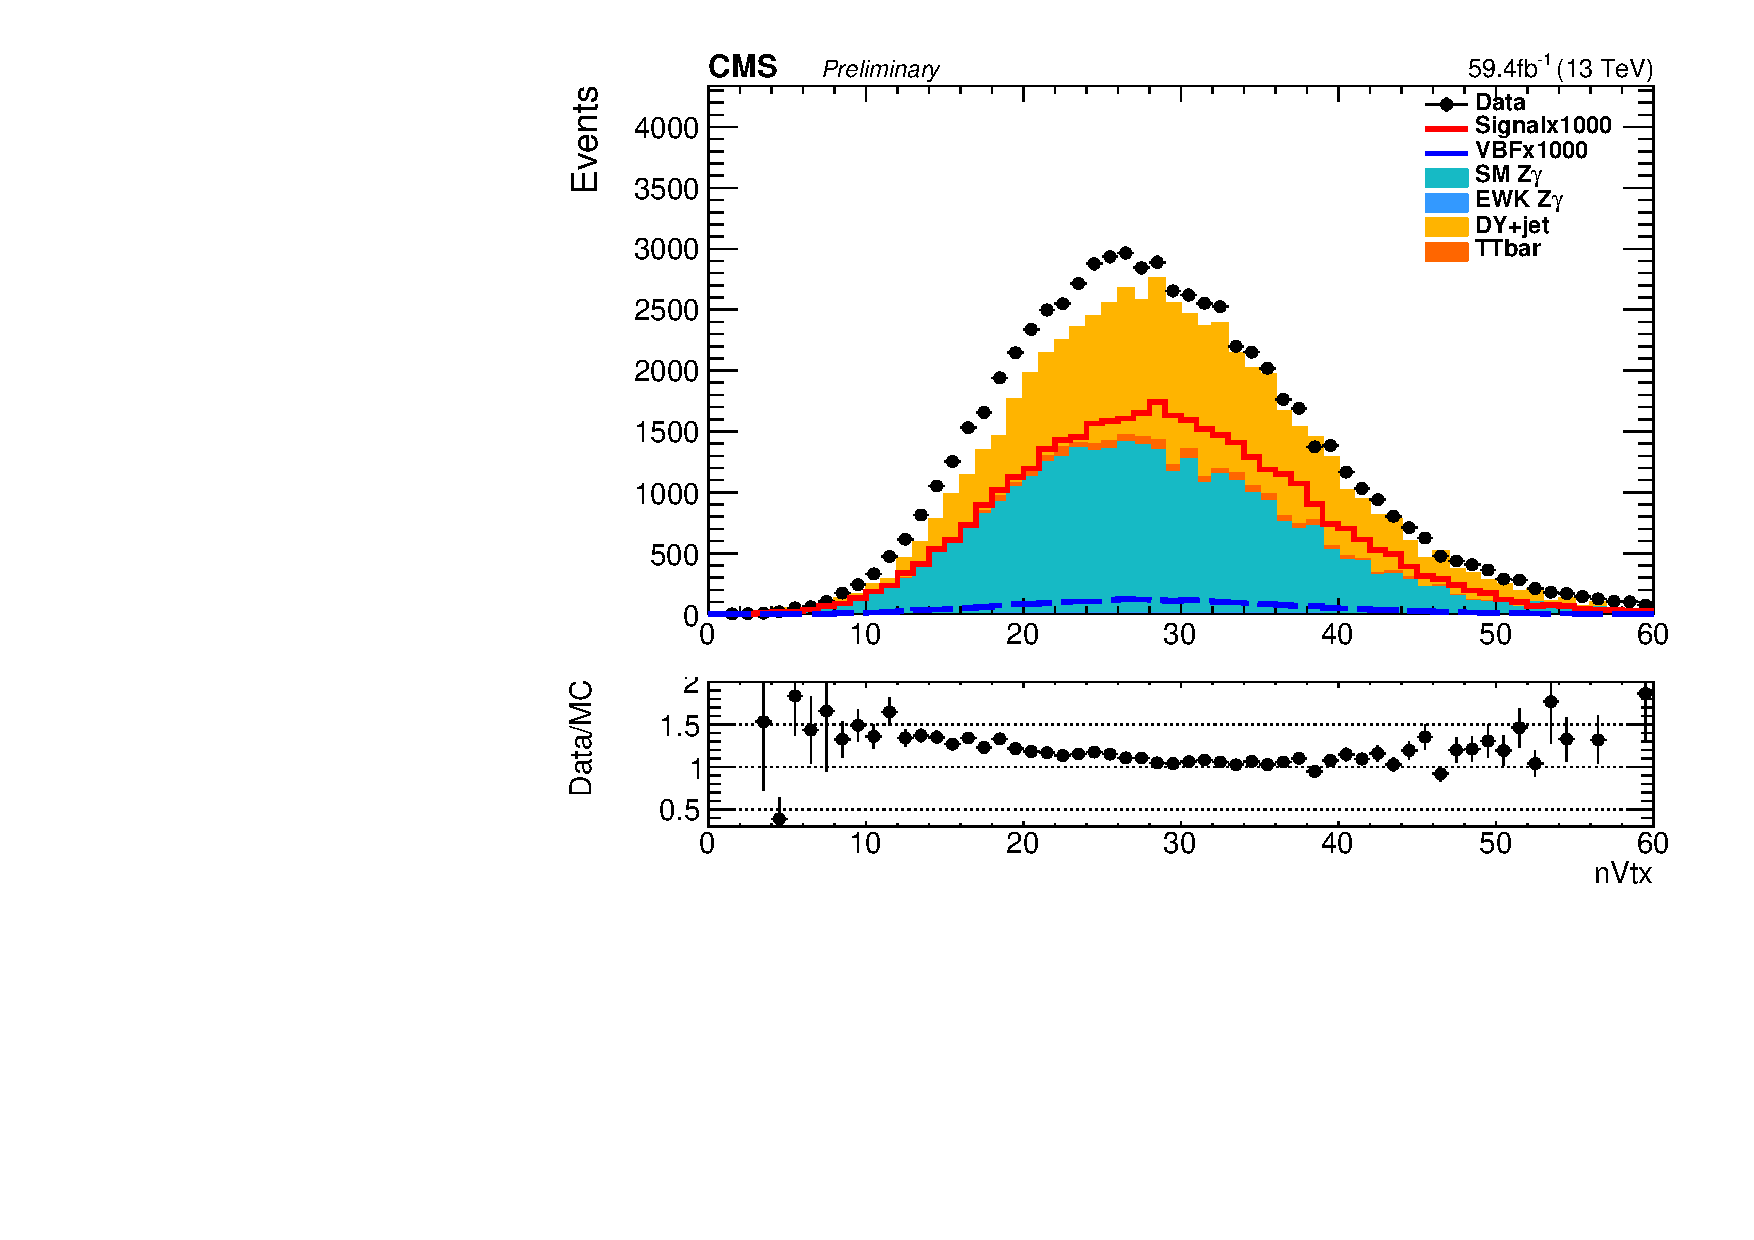
\includegraphics[width=0.3\textwidth]{fig/pileup/ele_kin_nVtx_valid_Rereco18_HLT.pdf}
  \end{center}
	\caption{Distributions of the number of primary vertices in data and simulation for $\epem\PGg$ events in 2016 (left), 2017 (center), and 2018 (right) after pileup reweighting.}
\label{fig:puwei}
\end{figure}

\section{Level-1 Trigger Prefiring Reweighting}\label{sec:L1}
In 2016 and 2017, a gradual timing shift of the ECAL was not properly propagated to 
L1 trigger primitives, resulting in a significant fraction of high-pseudorapidity trigger primitives
mistakenly associated to the previous bunch crossing~\cite{L1_prefire}. 
Since L1 trigger rules forbid two consecutive bunch crossings from triggering, 
a consequence is that events can self-veto if a significant amount of ECAL energy is found in the region 
$2<|\eta|<3$. This effect is not described in simulation.
To handle this, a weight is applied to each simulated event based on the probability of an event not to prefire and self-veto. 
The prefiring probability is determined by measuring the timing distributions of physics objects in the subset of data events for which prefiring 
is impossible due to the lack of a L1 trigger accept in the previous bunch crossing. The measurement is parameterized in 
$\eta$ and \pt. The final event weight applied to the simulation is the product of the non-prefiring probability of all objects, as shown in equation~\ref{eqn:prefire}.
\begin{equation}
	\omega = 1 - \mathrm{P(Prefiring)} = \prod_{i=\mathrm{photons,\,jets,\,muons}}(1-\epsilon_i^{\mathrm{pref}}(\eta,\pt^{\mathrm{EM,\,\mu}}))
	\label{eqn:prefire}
\end{equation}
The impact of the L1 prefiring for electrons (muons) is a 1.4 (0.8)\% loss in signal yield for 2016 and 2.4 (1.1)\% loss in signal yield for 2017.
The uncertainties associated with the L1 prefiring reweighting are accounted for in the analysis and are discussed further in Chapter~\ref{sec:uncertainties}.
